% Definir colores RACI
\definecolor{Rcolor}{RGB}{0, 51, 102} % Azul oscuro
\definecolor{Acolor}{RGB}{0, 102, 0}  % Verde oscuro
\definecolor{Ccolor}{RGB}{102, 51, 0} % Marrón oscuro
\definecolor{Icolor}{RGB}{189, 0, 0}  % Rojo oscuro

En el contexto del desarrollo del proyecto, se ha procedido a la identificación y análisis de los perfiles profesionales implicados, así como de las respectivas responsabilidades 
y tareas asignadas a cada uno. Aunque la ejecución del proyecto se realizará de forma individual, 
esta estructuración permite una asignación y gestión presupuestaria más precisa, alineando los recursos financieros con las funciones específicas requeridas para cada etapa del proyecto. 
Los roles se han representado por medio de la estructura jerárquica OBS (\textit{Organizational Breakdown Structure}), 
mostrada en la \coloredUnderline{\hyperlink{fig:obs}{Figura: \ref*{fig:obs} \nameref*{fig:obs}}}, 
faiclitando la visualización de la estructura organizativa del proyecto.

\begin{figure}[H]
    \centering
    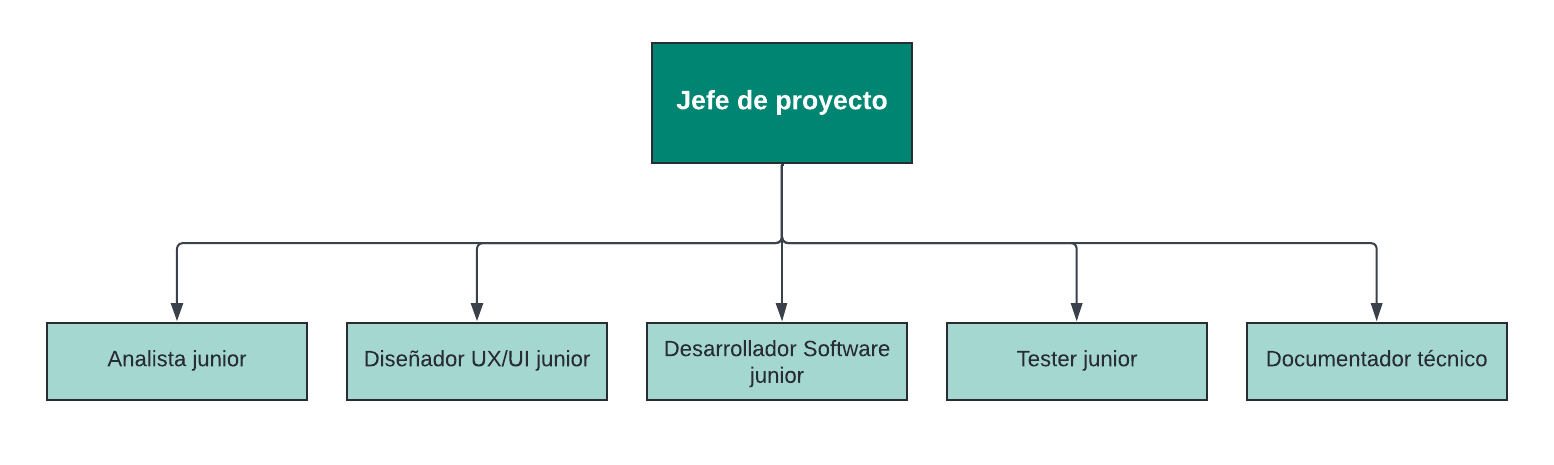
\includegraphics[width=0.8\textwidth]{figures/5_OBS.png}
    \caption{OBS del proyecto}
    \label{fig:obs}
    \hypertarget{fig:obs}{}
\end{figure}



Se ha decidido realizar una matriz de asignación de responsabilidades RACI para relacionar las tareas identifcadas en \coloredUnderline{\hyperlink{sec:5-WBS}{\ref*{sec:5-WBS} \nameref*{sec:5-WBS}}} con cada rol.
En esta matriz, a cada tarea se le asigna un rol con una de las siguientes responsabilidades:
\begin{itemize}
    \item \textbf{\textcolor{Rcolor}{R}:} Responsable. Persona que realiza la tarea.
    \item \textbf{\textcolor{Acolor}{A}:} Aprobador. Persona que aprueba la tarea.
    \item \textbf{\textcolor{Ccolor}{C}:} Consultado. Persona a la que se consulta sobre la tarea.
    \item \textbf{\textcolor{Icolor}{I}:} Informado. Persona a la que se informa sobre el avance y los resultados de la tarea.
\end{itemize}
Un mismo recurso puede tener varias responsabilidades en una misma tarea, en tal caso se anotarán separadas por el caracter ``/''. 
Los recursos que no tienen ninguna responsabilidad en una tarea se dejan en blanco.
En la tabla \coloredUnderline{\hyperlink{table:recursos}{Tabla \ref*{table:recursos}: \nameref*{table:recursos}}}, se muestran los roles y las abreviaturas utilizadas en la matriz RACI.

\begin{table}[H]
\centering
\hypertarget{table:recursos}{}
\caption{Roles y abreviaturas de los recursos}
\label{table:recursos}
\begin{tabular}{>{\columncolor{lightgreen!20}}p{2.2cm} p{6cm}}
\toprule
\rowcolor{darkgreen!50}
\textbf{Abreviatura} & \textbf{Rol} \\
\midrule
JP & Jefe de Proyecto \\
\midrule
AN & Analista junior\\
\midrule
DI & Diseñador junior \\
\midrule
DS & Desarrollador de Software junior\\
\midrule
TE & Tester junior \\
\midrule
DOC & Documentador técnico \\
\bottomrule
\end{tabular}
\end{table}
 

\subsubsubsection{Análisis del proyecto}
En la \coloredUnderline{\hyperlink{table:matriz-analisis}{Tabla: \ref*{table:matriz-analisis} \nameref*{table:matriz-analisis}}} se muestra la matriz de responsabilidades para la fase de análisis.
\begin{table}[H]
    \centering
    \caption{Tabla RACI de la fase Análisis del proyecto}
    \label{table:matriz-analisis}
    \hypertarget{table:matriz-analisis}{}
    \begin{tabular}{
    >{\columncolor{lightgreen!20}}m{7cm} 
    >{\columncolor{white}}m{1cm} 
    >{\columncolor{white}}m{1cm} 
    >{\columncolor{white}}m{1cm} 
    >{\columncolor{white}}m{1cm} 
    >{\columncolor{white}}m{1cm} 
    >{\columncolor{white}}m{1cm}}
    \cmidrule(l){2-7}
    \rowcolor{darkgreen!50}
    \cellcolor{white} & \multicolumn{6}{c}{\textbf{Roles}} \\
    \midrule
    \rowcolor{lightgreen!20}
    \cellcolor{darkgreen!50}\textbf{Tarea} & \textbf{JP} & \textbf{AN} & \textbf{DI} & \textbf{DS} & \textbf{TE} & \textbf{DOC} \\
    \midrule
    Análisis del sistema & \textbf{\textcolor{Acolor}{A}} & \textbf{\textcolor{Rcolor}{R} }&  & \textbf{\textcolor{Ccolor}{C}} &  &  \\
    \midrule
    Análisis de la arquitectura & \textbf{\textcolor{Acolor}{A}} & \textbf{\textcolor{Rcolor}{R}}&  & \textbf{\textcolor{Ccolor}{C}} &  &  \\
    \midrule
    Análisis de la infraestructura & \textbf{\textcolor{Acolor}{A}} & \textbf{\textcolor{Rcolor}{R}} &  & \textbf{\textcolor{Ccolor}{C} }&  &  \\
    \midrule
    Determinación del alcance de desarrollo & \textbf{\textcolor{Acolor}{A}} & \textbf{\textcolor{Rcolor}{R}} & \textbf{\textcolor{Icolor}{I}} & \textbf{\textcolor{Ccolor}{C}} & \textbf{\textcolor{Icolor}{I}} & \textbf{\textcolor{Icolor}{I}} \\
    \bottomrule
    \end{tabular}
\end{table}

\subsubsubsection{Seguimiento del proyecto}
En la \coloredUnderline{\hyperlink{table:matriz-seguimiento}{Tabla: \ref*{table:matriz-seguimiento} \nameref*{table:matriz-seguimiento}}} se muestra la matriz de responsabilidades para la fase de seguimiento.
\begin{table}[H]
    \centering
    \caption{Tabla RACI de la fase Seguimiento del proyecto}
    \label{table:matriz-seguimiento}
    \hypertarget{table:matriz-seguimiento}{}
    \begin{tabular}{
    >{\columncolor{lightgreen!20}}m{7cm} 
    >{\columncolor{white}}m{1cm} 
    >{\columncolor{white}}m{1cm} 
    >{\columncolor{white}}m{1cm} 
    >{\columncolor{white}}m{1cm} 
    >{\columncolor{white}}m{1cm} 
    >{\columncolor{white}}m{1cm}}
    \cmidrule(l){2-7}
    \rowcolor{darkgreen!50}
    \cellcolor{white} & \multicolumn{6}{c}{\textbf{Roles}} \\
    \midrule
    \rowcolor{lightgreen!20}
    \cellcolor{darkgreen!50}\textbf{Tarea} & \textbf{JP} & \textbf{AN} & \textbf{DI} & \textbf{DS} & \textbf{TE} & \textbf{DOC} \\
    \midrule
    Reunión de arranque & \textbf{\textcolor{Acolor}{A}} & \textbf{\textcolor{Ccolor}{C}} & \textbf{\textcolor{Icolor}{I}} & \textbf{\textcolor{Icolor}{I}} & \textbf{\textcolor{Icolor}{I}} & \textbf{\textcolor{Rcolor}{R}} \\
    \midrule
    Reuniones periódicas & \textbf{\textcolor{Acolor}{A}} & \textbf{\textcolor{Icolor}{I}} & \textbf{\textcolor{Icolor}{I}} & \textbf{\textcolor{Ccolor}{C}} & \textbf{\textcolor{Icolor}{I}} & \textbf{\textcolor{Rcolor}{R}} \\
    \midrule
    Reunión de revisión & \textbf{\textcolor{Acolor}{A}} & \textbf{\textcolor{Icolor}{I}} & \textbf{\textcolor{Icolor}{I}} & \textbf{\textcolor{Ccolor}{C}} & \textbf{\textcolor{Icolor}{I}} & \textbf{\textcolor{Rcolor}{R}} \\
    \midrule
    Reunión final & \textbf{\textcolor{Acolor}{A}} & \textbf{\textcolor{Icolor}{I}} & \textbf{\textcolor{Icolor}{I}} & \textbf{\textcolor{Ccolor}{C}} & \textbf{\textcolor{Icolor}{I}} & \textbf{\textcolor{Rcolor}{R}} \\
    \bottomrule
    \end{tabular}
\end{table}

\subsubsubsection{Diseño del sistema}
En la \coloredUnderline{\hyperlink{table:matriz-diseno}{Tabla: \ref*{table:matriz-diseno} \nameref*{table:matriz-diseno}}} se presenta la matriz de responsabilidades correspondiente a la fase de diseño. 
Las tareas listadas en esta matriz son las tareas "hoja" de dicha fase, es decir, aquellas que no se descomponen en subtareas más pequeñas y, por lo tanto, representan las tareas finales 
de la fase de diseño.
\begin{table}[H]
    \centering
    \caption{Tabla RACI de la fase Diseño del sistema}
    \label{table:matriz-diseno}
    \hypertarget{table:matriz-diseno}{}
    \begin{tabular}{
    >{\columncolor{lightgreen!20}}m{7cm} 
    >{\columncolor{white}}m{1cm} 
    >{\columncolor{white}}m{1cm} 
    >{\columncolor{white}}m{1cm} 
    >{\columncolor{white}}m{1cm} 
    >{\columncolor{white}}m{1cm} 
    >{\columncolor{white}}m{1cm}}
    \cmidrule(l){2-7}
    \rowcolor{darkgreen!50}
    \cellcolor{white} & \multicolumn{6}{c}{\textbf{Roles}} \\
    \midrule
    \rowcolor{lightgreen!20}
    \cellcolor{darkgreen!50}\textbf{Tarea} & \textbf{JP} & \textbf{AN} & \textbf{DI} & \textbf{DS} & \textbf{TE} & \textbf{DOC} \\
    \midrule
    \textit{Backend}. Diseño del módulo de usuarios & \textbf{\textcolor{Acolor}{A}} &  & \textbf{\textcolor{Icolor}{I}} & \textbf{\textcolor{Rcolor}{R}} &  &  \textbf{\textcolor{Icolor}{I}} \\
    \midrule
    \textit{Backend}. Diseño del módulo de cartas & \textbf{\textcolor{Acolor}{A}} &  & \textbf{\textcolor{Icolor}{I}} & \textbf{\textcolor{Rcolor}{R}} &  & \textbf{\textcolor{Icolor}{I}} \\
    \midrule
    \textit{Backend}. Diseño del módulo de sobres de cartas & \textbf{\textcolor{Acolor}{A}} &  & \textbf{\textcolor{Icolor}{I}} & \textbf{\textcolor{Rcolor}{R}} &  & \textbf{\textcolor{Icolor}{I}} \\
    \midrule
    \textit{Backend}. Diseño del módulo de subastas & \textbf{\textcolor{Acolor}{A}} &  & \textbf{\textcolor{Icolor}{I}} & \textbf{\textcolor{Rcolor}{R}} &  & \textbf{\textcolor{Icolor}{I}} \\
    \midrule
    \textit{Backend}. Diseño del módulo de transacciones & \textbf{\textcolor{Acolor}{A}} &  & \textbf{\textcolor{Icolor}{I}} & \textbf{\textcolor{Rcolor}{R}} &  & \textbf{\textcolor{Icolor}{I}} \\
    \midrule
    \textit{Frontend}. Diseño de logo de la aplicación & \textbf{\textcolor{Acolor}{A}} &  & \textbf{\textcolor{Rcolor}{R}} & \textbf{\textcolor{Icolor}{I}} &  & \textbf{\textcolor{Icolor}{I}} \\
    \midrule
    \textit{Frontend}. Diseño de la moneda de la aplicación & \textbf{\textcolor{Acolor}{A}} &  & \textbf{\textcolor{Rcolor}{R}} & \textbf{\textcolor{Icolor}{I}} &  & \textbf{\textcolor{Icolor}{I}} \\
    \midrule
    \textit{Frontend}. Diseño de la temática & \textbf{\textcolor{Acolor}{A}} &  & \textbf{\textcolor{Rcolor}{R}} & \textbf{\textcolor{Ccolor}{C}/\textcolor{Icolor}{I}} &  & \textbf{\textcolor{Icolor}{I}} \\
    \midrule
    \textit{Frontend}. Diseño del árbol de navegación & \textbf{\textcolor{Acolor}{A}} &  & \textbf{\textcolor{Rcolor}{R}} & \textbf{\textcolor{Ccolor}{C}/\textcolor{Icolor}{I}} &  & \textbf{\textcolor{Icolor}{I}} \\
    \midrule
    \textit{Frontend}. Diseño de las páginas de información & \textbf{\textcolor{Acolor}{A}} &  & \textbf{\textcolor{Rcolor}{R}} & \textbf{\textcolor{Ccolor}{C}/\textcolor{Icolor}{I}} &  & \textbf{\textcolor{Icolor}{I}} \\
    \midrule
    \textit{Frontend}. Diseño de la página \textit{Home} & \textbf{\textcolor{Acolor}{A}} &  & \textbf{\textcolor{Rcolor}{R}} & \textbf{\textcolor{Ccolor}{C}/\textcolor{Icolor}{I}} &  & \textbf{\textcolor{Icolor}{I}} \\
    \midrule
    \textit{Frontend}. Diseño de la página de error & \textbf{\textcolor{Acolor}{A}} &  & \textbf{\textcolor{Rcolor}{R}} & \textbf{\textcolor{Ccolor}{C}/\textcolor{Icolor}{I}} &  & \textbf{\textcolor{Icolor}{I}} \\
    \midrule
    \textit{Frontend}. Diseño del módulo de usuarios & \textbf{\textcolor{Acolor}{A}} &  & \textbf{\textcolor{Rcolor}{R}} & \textbf{\textcolor{Ccolor}{C}/\textcolor{Icolor}{I}} &  & \textbf{\textcolor{Icolor}{I}} \\
    \midrule
    \textit{Frontend}. Diseño del módulo de cartas & \textbf{\textcolor{Acolor}{A}} &  & \textbf{\textcolor{Rcolor}{R}} & \textbf{\textcolor{Ccolor}{C}/\textcolor{Icolor}{I}} &  & \textbf{\textcolor{Icolor}{I}} \\
    \midrule
    \textit{Frontend}. Diseño del módulo de sobres de cartas & \textbf{\textcolor{Acolor}{A}} &  & \textbf{\textcolor{Rcolor}{R}} & \textbf{\textcolor{Ccolor}{C}/\textcolor{Icolor}{I}} &  & \textbf{\textcolor{Icolor}{I}} \\
    \midrule
    \textit{Frontend}. Diseño del módulo de subastas & \textbf{\textcolor{Acolor}{A}} &  & \textbf{\textcolor{Rcolor}{R}} & \textbf{\textcolor{Ccolor}{C}/\textcolor{Icolor}{I}} &  & \textbf{\textcolor{Icolor}{I}} \\
    \midrule
    \textit{Frontend}. Diseño del módulo de transacciones & \textbf{\textcolor{Acolor}{A}} &  & \textbf{\textcolor{Rcolor}{R}} & \textbf{\textcolor{Ccolor}{C}/\textcolor{Icolor}{I}} &  & \textbf{\textcolor{Icolor}{I}} \\
    \midrule
    Diseño de la pruebas unitarias & \textbf{\textcolor{Acolor}{A}} &  & & \textbf{\textcolor{Ccolor}{C}/\textcolor{Icolor}{I}} & \textbf{\textcolor{Rcolor}{R}} & \textbf{\textcolor{Icolor}{I}} \\
    \midrule
    Diseño de la pruebas de carga/estrés & \textbf{\textcolor{Acolor}{A}} &  & & \textbf{\textcolor{Ccolor}{C}/\textcolor{Icolor}{I}} & \textbf{\textcolor{Rcolor}{R}} & \textbf{\textcolor{Icolor}{I}} \\
    \midrule
    Diseño de la pruebas \textit{end-to-end} & \textbf{\textcolor{Acolor}{A}} &  & & \textbf{\textcolor{Ccolor}{C}/\textcolor{Icolor}{I}} & \textbf{\textcolor{Rcolor}{R}} & \textbf{\textcolor{Icolor}{I}} \\
    \bottomrule
    \end{tabular}
\end{table}

\subsubsubsection{Implementación del sistema}
En la \coloredUnderline{\hyperlink{table:matriz-implementacion}{Tabla: \ref*{table:matriz-implementacion} \nameref*{table:matriz-implementacion}}} se muestra la matriz de responsabilidades para la fase de implementación.
Igual que en el caso anterior, las tareas listadas en esta matriz son las tareas finales de dicha fase.
\begin{longtable}{
    >{\columncolor{lightgreen!20}}m{7cm} 
    >{\columncolor{white}}m{1cm} 
    >{\columncolor{white}}m{1cm} 
    >{\columncolor{white}}m{1cm} 
    >{\columncolor{white}}m{1cm} 
    >{\columncolor{white}}m{1cm} 
    >{\columncolor{white}}m{1cm} }
    \caption{Tabla RACI de la fase Implementación del sistema} \label{table:matriz-implementacion}
    \hypertarget{table:matriz-implementacion}{}
    \\
    \cmidrule(l){2-7}
    \rowcolor{darkgreen!50}
    \cellcolor{white} & \multicolumn{6}{c}{\textbf{Roles}} \\
    \midrule
    \rowcolor{lightgreen!20}
    \cellcolor{darkgreen!50}\textbf{Tarea} & \textbf{JP} & \textbf{AN} & \textbf{DI} & \textbf{DS} & \textbf{TE} & \textbf{DOC} \\
    \endfirsthead

    \cmidrule(l){2-7}
    \rowcolor{darkgreen!50}
    \cellcolor{white} & \multicolumn{6}{c}{\textbf{Roles}} \\
    \midrule
    \rowcolor{lightgreen!20}
    \cellcolor{darkgreen!50}\textbf{Tarea} & \textbf{JP} & \textbf{AN} & \textbf{DI} & \textbf{DS} & \textbf{TE} & \textbf{DOC} \\
    \endhead

    \midrule
    \multicolumn{7}{r}{{Continúa en la siguiente página\ldots}} \\
    \endfoot

    \endlastfoot

    \textit{Backend}. Implementación del módulo de usuarios & \textbf{\textcolor{Acolor}{A}} &  &  & \textbf{\textcolor{Rcolor}{R}} & \textbf{\textcolor{Icolor}{I}} &  \textbf{\textcolor{Icolor}{I}} \\
    \midrule
    \textit{Backend}. Implementación del módulo de cartas & \textbf{\textcolor{Acolor}{A}} &  &  & \textbf{\textcolor{Rcolor}{R}} & \textbf{\textcolor{Icolor}{I}} & \textbf{\textcolor{Icolor}{I}} \\
    \midrule
    \textit{Backend}. Implementación del módulo de sobres de cartas & \textbf{\textcolor{Acolor}{A}} &  &  & \textbf{\textcolor{Rcolor}{R}} & \textbf{\textcolor{Icolor}{I}} & \textbf{\textcolor{Icolor}{I}} \\
    \midrule
    \textit{Backend}. Implementación del módulo de subastas & \textbf{\textcolor{Acolor}{A}} &  &  & \textbf{\textcolor{Rcolor}{R}} & \textbf{\textcolor{Icolor}{I}} & \textbf{\textcolor{Icolor}{I}} \\
    \midrule
    \textit{Backend}. Implementación del módulo de transacciones & \textbf{\textcolor{Acolor}{A}} &  &  & \textbf{\textcolor{Rcolor}{R}} & \textbf{\textcolor{Icolor}{I}} & \textbf{\textcolor{Icolor}{I}} \\
    \midrule
    \textit{Frontend}. Implementación de la temática & \textbf{\textcolor{Acolor}{A}} &  & \textbf{\textcolor{Ccolor}{C}} & \textbf{\textcolor{Rcolor}{R}} &  & \textbf{\textcolor{Icolor}{I}} \\
    \midrule
    \textit{Frontend}. Implementación de las rutas de navegación & \textbf{\textcolor{Acolor}{A}} &  & \textbf{\textcolor{Ccolor}{C}} & \textbf{\textcolor{Rcolor}{R}} & \textbf{\textcolor{Icolor}{I}} & \textbf{\textcolor{Icolor}{I}} \\
    \midrule
    \textit{Frontend}. Implementación de las páginas de información & \textbf{\textcolor{Acolor}{A}} &  & \textbf{\textcolor{Ccolor}{C}} & \textbf{\textcolor{Rcolor}{R}} & \textbf{\textcolor{Icolor}{I}} & \textbf{\textcolor{Icolor}{I}} \\
    \midrule
    \textit{Frontend}. Implementación de la página \textit{Home} & \textbf{\textcolor{Acolor}{A}} &  & \textcolor{Ccolor}{C} & \textbf{\textcolor{Rcolor}{R}} & \textbf{\textcolor{Icolor}{I}} & \textbf{\textcolor{Icolor}{I}} \\
    \midrule
    \textit{Frontend}. Implementación de la página de error & \textbf{\textcolor{Acolor}{A}} &  & \textbf{\textcolor{Ccolor}{C}} & \textbf{\textcolor{Rcolor}{R}} & \textbf{\textcolor{Icolor}{I}} & \textbf{\textcolor{Icolor}{I}} \\
    \midrule
    \textit{Frontend}. Implementación del módulo de usuarios & \textbf{\textcolor{Acolor}{A}} &  & \textbf{\textcolor{Ccolor}{C}} & \textbf{\textcolor{Rcolor}{R}} & \textbf{\textcolor{Icolor}{I}} & \textbf{\textcolor{Icolor}{I}} \\
    \midrule
    \textit{Frontend}. Implementación del módulo de cartas & \textbf{\textcolor{Acolor}{A}} &  & \textbf{\textcolor{Ccolor}{C}} & \textbf{\textcolor{Rcolor}{R}} & \textbf{\textcolor{Icolor}{I}} & \textbf{\textcolor{Icolor}{I}} \\
    \midrule
    \textit{Frontend}. Implementación del módulo de sobres de cartas & \textbf{\textcolor{Acolor}{A}} &  & \textbf{\textcolor{Ccolor}{C}} & \textbf{\textcolor{Rcolor}{R}} & \textbf{\textcolor{Icolor}{I}} & \textbf{\textcolor{Icolor}{I}} \\
    \midrule
    \textit{Frontend}. Implementación del módulo de subastas & \textbf{\textcolor{Acolor}{A}} &  & \textbf{\textcolor{Ccolor}{C}} & \textbf{\textcolor{Rcolor}{R}} & \textbf{\textcolor{Icolor}{I}} & \textbf{\textcolor{Icolor}{I}} \\
    \midrule
    \textit{Frontend}. Implementación del módulo de transacciones & \textbf{\textcolor{Acolor}{A}} &  & \textbf{\textcolor{Ccolor}{C}} & \textbf{\textcolor{Rcolor}{R}} & \textbf{\textcolor{Icolor}{I}} & \textbf{\textcolor{Icolor}{I}} \\
    \midrule
    Conexión \textit{backend}-\textit{frontend} & \textbf{\textcolor{Acolor}{A}} &  &  & \textbf{\textcolor{Rcolor}{R}} & \textbf{\textcolor{Icolor}{I}} & \textbf{\textcolor{Icolor}{I}} \\
    \midrule
    Implementación de la pruebas unitarias & \textbf{\textcolor{Acolor}{A}} &  &  & \textbf{\textcolor{Ccolor}{C}/\textcolor{Icolor}{I}} & \textbf{\textcolor{Rcolor}{R}} & \textbf{\textcolor{Icolor}{I}} \\
    \midrule
    Implementación de la pruebas de carga/estrés & \textbf{\textcolor{Acolor}{A}} &  &  & \textbf{\textcolor{Ccolor}{C}/\textcolor{Icolor}{I}} & \textbf{\textcolor{Rcolor}{R}} & \textbf{\textcolor{Icolor}{I}} \\
    \midrule
    Implementación de la pruebas \textit{end-to-end} & \textbf{\textcolor{Acolor}{A}} &  &  & \textbf{\textcolor{Ccolor}{C}/\textcolor{Icolor}{I}} & \textbf{\textcolor{Rcolor}{R}} & \textbf{\textcolor{Icolor}{I}} \\
    \bottomrule
\end{longtable}

\subsubsubsection{Fase de pruebas}
A continuación, se detallan las responsabilidades de cada rol en la fase de pruebas del sistema. 
En la \coloredUnderline{\hyperlink{table:matriz-pruebas}{Tabla: \ref*{table:matriz-pruebas} \nameref*{table:matriz-pruebas}}}, se muestra la matriz de responsabilidades para la fase de pruebas.
\begin{table}[H]
    \centering
    \caption{Tabla RACI de la Fase de pruebas}
    \label{table:matriz-pruebas}
    \hypertarget{table:matriz-pruebas}{}
    \begin{tabular}{
    >{\columncolor{lightgreen!20}}m{7 cm}
    >{\columncolor{white}}m{1cm}
    >{\columncolor{white}}m{1cm}
    >{\columncolor{white}}m{1cm}
    >{\columncolor{white}}m{1cm}
    >{\columncolor{white}}m{1cm}
    >{\columncolor{white}}m{1cm}}
    \cmidrule(l){2-7}
    \rowcolor{darkgreen!50}
    \cellcolor{white} & \multicolumn{6}{c}{\textbf{Roles}} \\
    \midrule
    \rowcolor{lightgreen!20}
    \cellcolor{darkgreen!50}\textbf{Tarea} & \textbf{JP} & \textbf{AN} & \textbf{DI} & \textbf{DS} & \textbf{TE} & \textbf{DOC} \\
    \midrule
    Ejecución de pruebas unitarias & \textbf{\textcolor{Acolor}{A}} &  &  & \textbf{\textcolor{Ccolor}{C}/\textcolor{Icolor}{I}} & \textbf{\textcolor{Rcolor}{R}} & \textbf{\textcolor{Icolor}{I}} \\
    \midrule
    Ejecución de pruebas de carga/estrés & \textbf{\textcolor{Acolor}{A}} &  &  & \textbf{\textcolor{Ccolor}{C}/\textcolor{Icolor}{I}} & \textbf{\textcolor{Rcolor}{R}} & \textbf{\textcolor{Icolor}{I}} \\
    \midrule
    Ejecución de pruebas \textit{end-to-end} & \textbf{\textcolor{Acolor}{A}} &  &  & \textbf{\textcolor{Ccolor}{C}/\textcolor{Icolor}{I}} & \textbf{\textcolor{Rcolor}{R}} & \textbf{\textcolor{Icolor}{I}} \\
    \bottomrule
    \end{tabular}
\end{table}

\subsubsubsection{Despliegue del sistema}
En la \coloredUnderline{\hyperlink{table:matriz-despliegue}{Tabla: \ref*{table:matriz-despliegue} \nameref*{table:matriz-despliegue}}}, se muestra la matriz de responsabilidades para la fase de despliegue.
\begin{table}[H]
    \centering
    \caption{Tabla RACI de la fase Despliegue del sistema}
    \label{table:matriz-despliegue}
    \hypertarget{table:matriz-despliegue}{}
    \begin{tabular}{
        >{\columncolor{lightgreen!20}}m{7cm} 
        >{\columncolor{white}}m{1cm} 
        >{\columncolor{white}}m{1cm} 
        >{\columncolor{white}}m{1cm} 
        >{\columncolor{white}}m{1cm} 
        >{\columncolor{white}}m{1cm} 
        >{\columncolor{white}}m{1cm}}
        \cmidrule(l){2-7}
        \rowcolor{darkgreen!50}
        \cellcolor{white} & \multicolumn{6}{c}{\textbf{Roles}} \\
        \midrule
        \rowcolor{lightgreen!20}
        \cellcolor{darkgreen!50}\textbf{Tarea} & \textbf{JP} & \textbf{AN} & \textbf{DI} & \textbf{DS} & \textbf{TE} & \textbf{DOC} \\
        \midrule
        Configuración del servidor Azure & \textbf{\textcolor{Acolor}{A}} & \textbf{\textcolor{Ccolor}{C}}  &  & \textbf{\textcolor{Rcolor}{R}} &  & \textbf{\textcolor{Icolor}{I}} \\
        \midrule
        Despliegue del sistema & \textbf{\textcolor{Acolor}{A}} &  &  & \textbf{\textcolor{Rcolor}{R}} &  & \textbf{\textcolor{Icolor}{I}} \\
        \bottomrule
    \end{tabular}
\end{table}

\subsubsubsection{Documentación del proyecto}
Por último, en la \coloredUnderline{\hyperlink{table:matriz-documentacion}{Tabla: \ref*{table:matriz-documentacion} \nameref*{table:matriz-documentacion}}}, se muestra la matriz de responsabilidades para la fase de documentación.
\begin{table}[H]
    \centering
    \caption{Tabla RACI de la fase Documentación del proyecto}
    \label{table:matriz-documentacion}
    \hypertarget{table:matriz-documentacion}{}
    \begin{tabular}{
        >{\columncolor{lightgreen!20}}m{7cm} 
        >{\columncolor{white}}m{1cm} 
        >{\columncolor{white}}m{1cm} 
        >{\columncolor{white}}m{1cm} 
        >{\columncolor{white}}m{1cm} 
        >{\columncolor{white}}m{1cm} 
        >{\columncolor{white}}m{1cm}}
        \cmidrule(l){2-7}
        \rowcolor{darkgreen!50}
        \cellcolor{white} & \multicolumn{6}{c}{\textbf{Roles}} \\
        \midrule
        \rowcolor{lightgreen!20}
        \cellcolor{darkgreen!50}\textbf{Tarea} & \textbf{JP} & \textbf{AN} & \textbf{DI} & \textbf{DS} & \textbf{TE} & \textbf{DOC} \\
        \midrule
        Creación de la plantilla LaTeX & \textbf{\textcolor{Acolor}{A}} &  &  & &  & \textbf{\textcolor{Rcolor}{R}} \\
        \midrule
        Redacción del documento final & \textbf{\textcolor{Acolor}{A}} &  &  & &  & \textbf{\textcolor{Rcolor}{R}}  \\
        \midrule
        Redacción de anexos & \textbf{\textcolor{Acolor}{A}} &  &  & &  & \textbf{\textcolor{Rcolor}{R}}  \\
        \midrule
        Presentación del proyecto & \textbf{\textcolor{Acolor}{A}} &  &  & &  & \textbf{\textcolor{Rcolor}{R}}  \\
        \bottomrule
    \end{tabular}
\end{table}